\begin{figure*}[t]
    \centering
    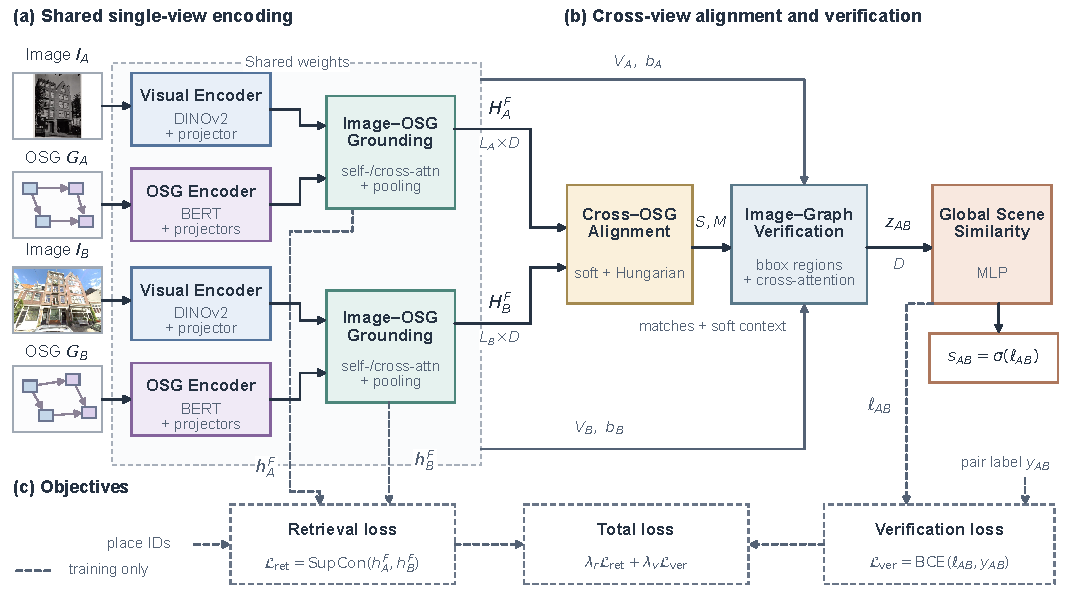
\includegraphics[width=\textwidth]{materials/figures/cosmic_framework.pdf}
    \caption{Overview of COSMIC. A shared single-view encoder extracts visual
    and BERT-based node/triplet features and grounds graph tokens in each image.
    The fused token set $H_X^F$ supports cross-view alignment, while its pooled
    descriptor $h_X^F$ supports independent retrieval. Type-aware soft alignment
    and partial Hungarian matching establish correspondences. Soft counterpart
    context guides bbox-based visual region verification, producing a symmetric
    pair embedding $z_{AB}$ and a same-place score $s_{AB}$. Dashed connections
    denote the supervised contrastive retrieval and binary pair-verification
    objectives; BCE receives raw logits before sigmoid. Input photographs show
    an illustrative AmsterTime pair; graph drawings are schematic.}
    \label{fig:cosmic-framework}
\end{figure*}
